%\chapter{The Patmos Compiler}
%\label{sec:compiler}


The Patmos compiler is an adaptation of the LLVM compiler~\cite{llvm:2004} to
target the Patmos processor ISA and to provide a tighter integration with WCET
analysis~\cite{Seus13:compiler}.

The compilation tool chain consists of the following components:

\begin{itemize}
\item \code{patmos-llvm} The compiler, including \code{platin} and various compiler tools, objdump and an assembler (patmos-llvm-mc).
\item \code{patmos-clang} The C frontend and the compiler/linker driver. Compiled together with patmos-llvm.
\item \code{patmos-gold} The \code{patmos-ld} ELF linker for Patmos.
\item \code{patmos-compiler-rt} The runtime library, defining software implementations of div and floats.
\item \code{patmos-newlib} The C library implementation.
\item \code{patmos-benchmarks} Various benchmarks that have been adapted to Patmos.
\item \code{patmos-misc} A collection of helper scripts for debugging, evaluation and building.
\item \code{patmos} The processor and the simulator.
\end{itemize}

The compiler and libraries can be built using \code{misc/build.sh} as described
in Section~\ref{sec:build:compiler}.  Details on building the tool chain
manually without the build script can be found in the \code{README.patmos}
files provided in the various repositories.


%%%%%%%%%%%%%%%%%%%%%%%%%%%%%%%%%%%%%%%%%%%%%%%%%%%%%%%%%%%%%%%%%%%%%%%%%%%%%%%
\section{Overview}

\begin{figure}[!t]
\centering
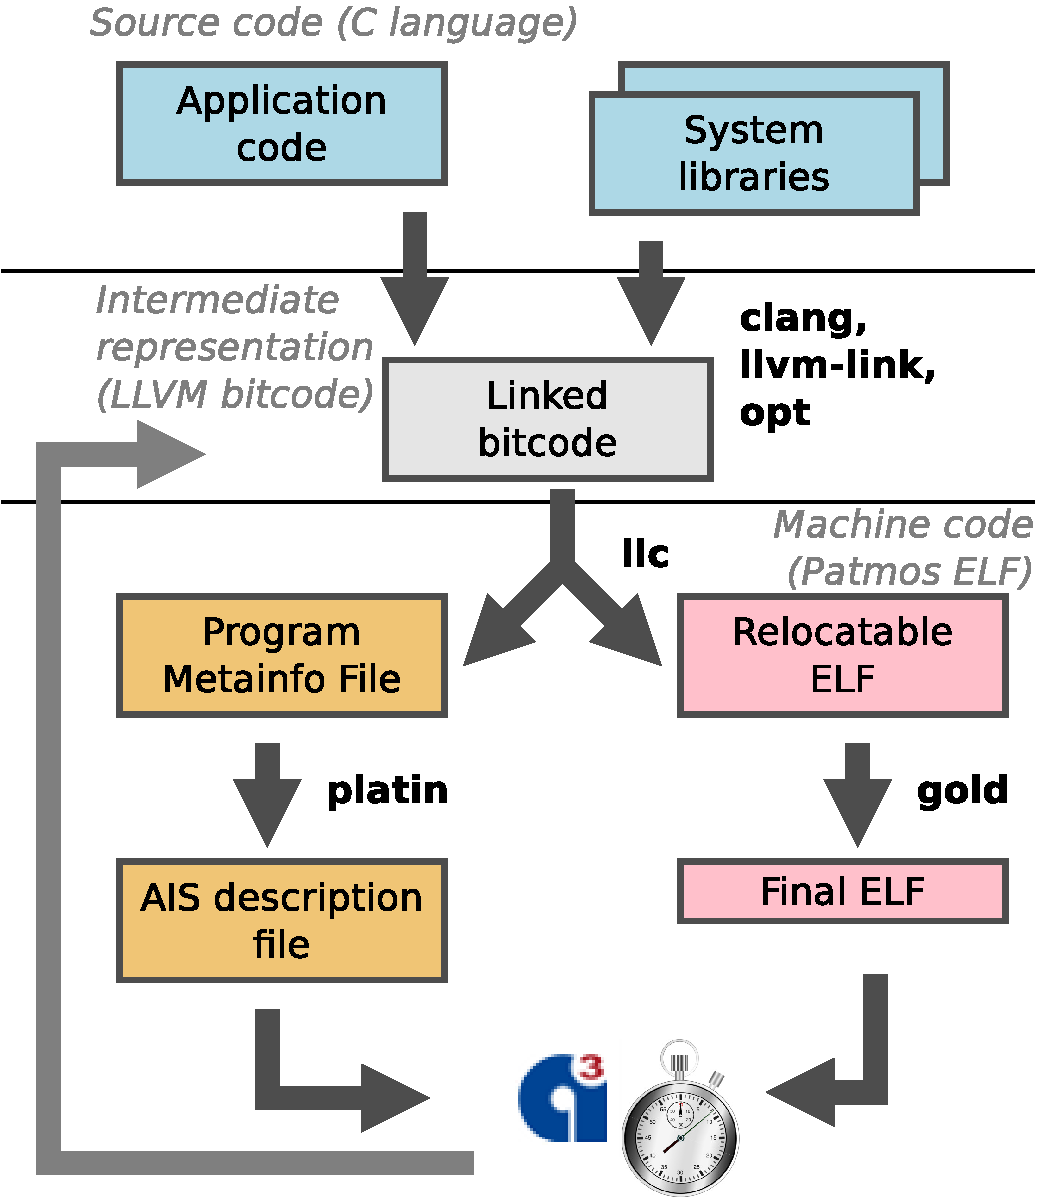
\includegraphics[width=0.5\textwidth]{fig/compiler_overview}
\caption{Compiler Tool Chain Overview}
\label{fig:compiler_overview}
\end{figure}


Figure~\ref{fig:compiler_overview} gives an overview of the compiler tool
chain.
The compilation process starts with the translation of each C source file and
libraries to the LLVM intermediate language (\emph{bitcode}) by the C frontend
\code{clang}. At this level, the user application code and static standard
and support libraries are linked by the \code{llvm-link} tool.
An advantage of linking on bitcode level is that subsequent analysis and
optimisation passes, and the code generation backend have a complete view of
the whole program. The \code{opt} optimiser performs generic,
target independent optimisations, such as common sub-expression elimination,
constant propagation, etc.

The \code{llc} tool constitutes the backend, translating LLVM bitcode into
machine code for the Patmos ISA, and addressing the target-specific features
for time predictability.  The backend produces a relocatable ELF binary
containing symbolic address information, which is processed by \code{gold}%
%
\footnote{gold is part of the GNU binutils, see
\url{http://sourceware.org/binutils/}}, defining the final data and memory
layout, and resolving symbol relocations.

In addition to the machine code, the backend exports supplementary information
for WCET analysis and optimisation purposes in form of a \emph{Patmos Metainfo
File}.  This information contains, among others, flow information (in form of
loop bounds provided by symbolic analysis on bitcode level), structural
information (targets of indirect branches), and information on memory accesses
(memory areas accessed by individual load/store instructions).
%
This information can be further processed by the \code{platin} toolkit, by
enhancing it (e.g., by a hardware model), translating it (e.g., to the input
format for annotations of the timing analysis tool \code{aiT}, as used in the
T-CREST project), or performing other analyses on it.





%%%%%%%%%%%%%%%%%%%%%%%%%%%%%%%%%%%%%%%%%%%%%%%%%%%%%%%%%%%%%%%%%%%%%%%%%%%%%%%
\section{Compiling with the \code{patmos-clang} Driver}

This section describes the usage of the \code{patmos-clang} C compiler.

\subsection{Compiling and Linking C Programs}

C source files are by default compiled to bitcode objects (\code{patmos-clang -c}). To compile .c files
to ELF objects, use \code{patmos-clang -c -fpatmos-emit-reloc}.

Assembly files are always compiled to ELF objects. Archive files (.a) can only contain bitcode objects
or ELF objects, not a mixture of both. Shared libraries (either bitcode or ELF) are not supported.

It is possible to link multiple bitcode files into a single bitcode file and link it like a static library
(compile with \code{patmos-clang -fpatmos-link-object -o lib<name>.bc}, link with -l<name>). Bitcode files are always
fully linked in, even if there is no usage of any of its symbols. Unused symbols are removed in a separate
optimization step.


\stefan{TODO Make the following a subsection. Describe interaction with platin, install directories layout of newlib. Show typical
compile commands using examples (compiling a single file, comiling a lib, compiling with platin,...}


\paragraph{Compiling single files to objects (using patmos-clang -c|-S)}

\begin{enumerate}
\item Input .c files are compiled to bitcode files by default. Use -fpatmos-emit-obj to compile
   to ELF objects, or -fpatmos-emit-asm to compile to assembly files.

\item Input .s files are compiled to ELF files.
\end{enumerate}


\paragraph{Linking multiple files with patmos-clang (i.e, not using -c or -S)}

The compiler driver (patmos-clang) performs the following steps to compile and link multiple input files.

\begin{enumerate}
\item All .c input files are compiled to individual bitcode objects. All assembly files are compiled to
   individual ELF files.

\item If -nostartfiles is not given and the target OS is not RTEMS, crt0 is added as first input file.

\item Depending on the -nodefaultlibs|-noruntimelibs|.. options, the following libraries are added
   after all user provided inputs: -lc (libc), -lpatmos (libgloss), -lrtsf (softfloats), -lrt (runtime).

\item For any of the above libraries, as well as -lm (libm), a lib<libname>syms.o file is added if the library
   is a bitcode library. The lib<x>syms.o files force the linker to pull in functions for which calls might be
   generated by LLC when compiling from bitcode to ELF.

\item All input files and libraries are checked if they are bitcode files/archives or ELF files/archives. All
   bitcode files are linked into a single bitcode file. ELF files are ignored in this step.

Attention: This means that symbols that are defined in bitcode archives but are used only in ELF input files
   are not linked in! You need to link in a separate bitcode file containing a pseudo use of the required symbols.

\item The resulting bitcode file is optimized and compiled to relocatable ELF.

Attention: The optimization step removes any symbol from the bitcode that are not used in bitcode.
   If a function is called only in an ELF object, you need to mark the function with \code{\_\_attribute\_\_((used))}.

\item The ELF file is linked with the other ELF files and ELF libraries at the position of the first bitcode input file.
   Relocations are resolved and additional symbols are defined. The result is an executable ELF file.

Attention: Since bitcode inputs are linked first in a separate step, the linking order between bitcode files
   and ELF inputs is not (yet) fully preserved. Using -flto does not solve this, since the LTO plugin also
   links all bitcode files first, and only links in the linked bitcode file *after* all ELF inputs!

\end{enumerate}

\subsubsection{Driver Options}

The \texttt{patmos-clang} driver can be used to generate bitcode files, to link bitcode files, or to 
emit assembler code. The driver supports the following modes of operation:

\begin{description}
\item[\texttt{patmos-clang -c <inputs>}] \hfill\\
  \begin{tabular}{ll}
  Input:   & \texttt{.c} C source file \\
  Output:  & \texttt{.o} or \texttt{.bc} bitcode files \\
  Actions: & compile each input file to a bitcode file
  \end{tabular}

\item[\texttt{patmos-clang -S <inputs>}] \hfill\\
  \begin{tabular}{ll}
  Input:   & \texttt{.c} C source file \\
  Output:  & \texttt{.s} or \texttt{.ll} human readable bitcode files \\
  Actions: & compile each input file to a human readable bitcode file
  \end{tabular}

\item[\texttt{patmos-clang -fpatmos-emit-llvm <inputs>}] \hfill\\
  \begin{tabular}{ll}
  Input:   & \texttt{.c} C source file, \texttt{.bc} bitcode object file, \texttt{.a} bitcode files archive \\
  Output:  & bitcode file \\
  Actions: & compile to bitcode, link all input files, link with standard libraries and start code \\
\end{tabular}

\item[\texttt{patmos-clang -fpatmos-emit-reloc -c <inputs>}] \hfill\\
  \begin{tabular}{ll}
  Input:   & \texttt{.c} C source file \\
  Output:  & \texttt{.o} Patmos relocatable ELF \\
  Actions: & compile each input file to a Patmos relocatable ELF file
  \end{tabular}

\item[\texttt{patmos-clang -fpatmos-emit-asm -S <inputs>}] \hfill\\
  \begin{tabular}{ll}
  Input:   & \texttt{.c} C source file \\
  Output:  & \texttt{.s} Patmos assembly file \\
  Actions: & compile each input file to a Patmos assembly file
  \end{tabular}

\item[\texttt{patmos-clang -fpatmos-emit-reloc <inputs>}] \hfill\\
  \begin{tabular}{ll}
  Input:   & \texttt{.c} C source file, \texttt{.bc} bitcode object file, \texttt{.a} bitcode files archive \\
  Output:  & \texttt{.o} Patmos relocatable ELF \\
  Actions: & compile to bitcode, link all input files, link with standard libraries and start code, \\
	   & compile to relocatable ELF
\end{tabular}

\item[\texttt{patmos-clang -fpatmos-emit-asm <inputs>}] \hfill\\
  \begin{tabular}{ll}
  Input:   & \texttt{.c} C source file, \texttt{.bc} bitcode object file, \texttt{.a} bitcode files archive \\
  Output:  & \texttt{.o} Patmos assembly file \\
  Actions: & compile to bitcode, link all input files, link with standard libraries and start code, \\
	   & compile to Patmos assembly
\end{tabular}

\item[\texttt{patmos-clang -o <output> <inputs>}] \hfill\\
  \begin{tabular}{ll}
  Input:   & \texttt{.c} C source file, \texttt{.bc} bitcode object file, \texttt{.a} bitcode files archive \\
  Output:  & Patmos executable ELF \\
  Actions: & compile to bitcode, link with standard libraries and start code, \\
           & compile to relocatable ELF, create Patmos executable ELF
  \end{tabular}

\end{description}

The compiler accepts standard options such as \texttt{-I}, \texttt{-L} and \texttt{-l} to define additional
lookup paths for header files and libraries and to link with (static) libraries.
The behaviour of the linker can be controlled with additional options for \texttt{patmos-clang} 
as shown in Table~\ref{tab:linker_options}.
Refer to \code{patmos-clang --help-hidden} for a list of all available options that control the behaviour of
the driver, and to \code{patmos-llc --help-hidden} for all options that control the generation of machine code from
bitcode. Options can be passed from \code{patmos-clang} to \code{patmos-llc} and other tools using \code{-Xclang},
\code{-Xopt}, \code{-Xllc}, \code{-Wl} and so on.
To pass options to the internal LLVM backend of the clang compiler, use \code{patmos-clang -Xclang -mllvm -Xclang
<option>}.

\begin{table}
\centering
\begin{tabular}{ll}
Option & Description \\ \hline
\texttt{-mfloat-abi=none} & Do not use software floating point libraries when linking \\
\texttt{-nostdlib} & Do not use standard libraries such as \texttt{libc} when linking \\
\texttt{-nolibc} & Do not use \texttt{libc} when linking \\
\texttt{-nodefaultlibs} & Do not use platform system libraries when linking\\
\texttt{-nostartfiles} & Do not use the \texttt{crt0} start file when linking \\
\texttt{-nolibsyms} & Do not use symbol definition files for runtime libraries when\\
                    & linking. Those files prevent the linker from removing any \\
		    & functions for which calls might be generated by the compiler \\
		    & backend, such as software division or \texttt{memcpy} \\
\texttt{-fpatmos-link-object} & Link as object, i.e., do not link in any libraries or start code 
\end{tabular}
\caption{Options for \texttt{patmos-clang} that control the default behaviour of the linker}
\label{tab:linker_options}
\end{table}

\subsubsection{Libraries}

The Patmos tool chain supports static libraries. Libraries are archives that contain
either only bitcode files or ELF objects. The archives are created by using either the \texttt{ar}
tool provided by the host system or by using \texttt{patmos-ar} from the \texttt{patmos-gold} binutils. The tool
\texttt{patmos-llvm-nm} can be used to inspect the content of bitcode archives.

\begin{verbatim}
ar q libtest.a *.bc
# show the contents of libtest.a
patmos-llvm-nm libtest.a
# compile and link with the created library
patmos-clang -target patmos-unknown-elf -o app main.c -ltest
\end{verbatim}


\subsection{Disassembling}

To disassemble .bc files, use \code{patmos-llvm-dis <file>.bc}.

To disassemble .o ELF files, use \code{patmos-llvm-objdump -d <file>}. Add '-r' to show relocation symbols
(for relocatable ELFs or executables generated with -Xgold -q).

\subsection{Debugging}

Some useful commands for debugging:

\begin{verbatim}
# print out executed instructions and the values of their operands
# starting from some cycle
pasim --debug=<cycle-to-start-printing> --debug-fmt=instr <binary>

# show disassembly of binary
patmos-llvm-objdump -r -d <binary> | less

# compile with debug infos, show source line numbers
patmos-clang -g -o <binary> ...
readelf --debug-dump=decodedline <binary>

# Compile with debugging info: use CFLAGS="-g" for your application, and add
# the following to your build.cfg:

NEWLIB_TARGET_CFLAGS="-g"
COMPILER_RT_CFLAGS="-g"

# Annotate objdump with source line numbes (this is quite slow at the moment)
patmos-llvm-objdump -r -d <binary> | patmos-dwarfdump <binary> | less

# Annotate simulation trace and stack-trace with line numbers
pasim --debug=<cycle-to-start-printing> --debug-fmt=instr <binary> 2>log.txt
cat log.txt | patmos-dwarfdump <binary>
\end{verbatim}

\subsection{Various options}

\paragraph{Keep relocation infos in executable for objdump:} (does not work with patmos-clang -g !)

\begin{verbatim}
patmos-clang -Xgold -q -o <binary> ....
patmos-llvm-objdump -r -d <binary> | less
\end{verbatim}




%%%%%%%%%%%%%%%%%%%%%%%%%%%%%%%%%%%%%%%%%%%%%%%%%%%%%%%%%%%%%%%%%%%%%%%%%%%%%%%
\section{\code{platin} -- The Portable LLVM Annotation and Timing Toolkit}
\label{sec:toolchain:platin}

The \code{platin} toolkit provides a set of useful tools to process the
information exported by the compiler in the PML format, with respect to
timing analysis integration.


The usage of \code{platin} is:

\begin{verbatim}
  platin <tool> <tool-options>
\end{verbatim}

You can get help on a particular tool with either of

\begin{verbatim}
  platin <tool> --help
  platin help <tool>
\end{verbatim}


Below we present a list of the most useful tools.

\begin{description}

  \item[pml2ais] \hfill\\
    Translates information of a PML file relevant to timing analysis to
    the AIS annotation format.

  \item[extract-symbols] \hfill\\
    The compiler exports program information at a stage where the final memory
    layout is not yet defined. This tool reads the final executable and
    enhances the PML file with information on the final addresses of
    instructions and data.

  \item[analyze-trace] \hfill\\
    Based on the structural information of a program in the PML file,
    the trace analysis tool is capable of extracting flow fact hypotheses
    based on a simulation run. These are context-sensitive and include,
    e.g.\ observed loop bounds and function call targets.

  \item[transform] \hfill\\
    Transforms flow facts from bitcode to machine code level
    or simplifies a set of flow facts.

  \item[tool-config] \hfill\\
    Given a hardware model (in PML format), this tool outputs consistent
    hardware configuration options/parameters for use during compilation,
    simulation and WCET analysis.

  \item[pml] \hfill\\
    Provides validation, inspection and merge facilities for PML files.

  \item[visualize] \hfill\\
    Visualises structural information of the program in the different program
    representations.

  \item[wcet] \hfill\\
    A driver that starts WCET analysis from the command line.

\end{description}


In addition to the platin tools, another command-line utility,
\texttt{patmos-clang-wcet}, is provided. This tool invokes the compiler
(\texttt{patmos-clang}), timing analysis, and the compiler a second time
(with intermediate calls to platin tools as necessary) for WCET-guided
optimisations based on timing-analysis feedback.
\daniel{TBD}

\subsection{The PML File Format}

\code{platin} stores all internal information and configuration in \emph{Platin Metainformation Language} (PML) files.
PML files are \emph{YAML} files that adhere to the PML schema. The schema file can be found in

\begin{verbatim}
patmos-llvm/tools/platin/lib/core/pml.yml
\end{verbatim}

\stefan{There is a tool to generate a HTML document out of it..}

Many \code{platin} tools accept multiple PML input files. Multiple PML files can also be merged using
the \code{pml} tool.

\subsection{PML Architecture- and Tool Configuration}

PML configuration files are used to set up tools such as the \code{pasim} or the
\code{clang} compiler via the \code{tool-config} tool, and provides timing and cache information to the WCET analyses.

Typically, the configuration is stored in a separate PML file that is passed to the \code{platin} tools as
additional input file using the \code{-i} option. Sample configuration files can be found in

\begin{verbatim}
patmos-llvm/tools/platin/etc/
\end{verbatim}
\stefan{Maybe we will install those files somewhere along with the .rb files.}




There are three configuration sections: 
\begin{itemize}
\item \code{machine-configuration}: The machine configuration defines memory size and timings, caches and memory areas.
  If no machine configuration is present, a default configuration will be used.
\item \code{tool-configurations}: This section contains additional tool configurations and options.
\item \code{analysis-configurations}: The analysis section sets up one or more WCET analyses. This section is currently work in progress.
\end{itemize}

\paragraph{The \code{machine-configuration} Section}


% TODO make this a figure or something. Maybe shorten?
\begin{verbatim}
---
format: pml-0.1
triple: patmos-unknown-unknown-elf
machine-configuration:
  memories:
    - name: "main"
      size: 0x200000
      transfer-size: 16
      read-latency: 3
      read-transfer-time: 4
      write-latency: 3
      write-transfer-time: 4
    - name: "local"
      size: 2048
      transfer-size: 4
      read-latency: 0
      read-transfer-time: 0
      write-latency: 0
      write-transfer-time: 0
  caches:
    - name: "data-cache"
      block-size: 16
      associativity: 1
      size: 2048
      policy: "lru"
      type: "set-associative"
    - name: "method-cache"
      block-size: 8
      associativity: 16
      size: 4096
      policy: "fifo"
      type: "method-cache"
    - name: "stack-cache"
      block-size: 4
      size: 2048
      type: "stack-cache"
  memory-areas:
    - name: "code"
      type: "code"
      memory: "main"
      cache: "method-cache"
      address-range:
        min: 0
        max: 0x200000
    - name: "data"
      type: "data"
      memory: "main"
      cache: "data-cache"
      address-range:
        min: 0
        max: 0x200000
      attributes:
        - key: "heap-end"
          value: 0x100000
        - key: "stack-base"
          value: 0x200000
        - key: "shadow-stack-base"
          value: 0x1f8000
\end{verbatim}


The machine configuration consists of three sections:
\begin{itemize}
\item \code{memories}: This section specifies the available memories and their timings. Each entry must define
  the following properties of the memory:

  \begin{itemize}
  \item \code{name}: The (unique) name of the memory.
  \item \code{size}: The size of the memory in bytes. Can be a hexadecimal value.
  \item \code{transfer-size}: The size of a single beat in bytes.

  \stefan{This should actually be more like the bus width and in bits, but this has historic reasons..}

  \item \code{min-burst-size}: The minimum size of a single burst in bytes. Defaults to \code{transfer-size}.
  \item \code{max-burst-size}: The maximum size of a single burst in bytes. Defaults to \code{min-burst-size}.
  
  \item \code{read-latency}: The latency per read \emph{request} in cycles.
  \item \code{read-transfer-time}: The number of cycles to read a single beat of size \code{transfer-size}.
  \item \code{write-latency}: The latency per write \emph{request} in cycles.
  \item \code{write-transfer-time}: The number of cycles to write a single beat of size \code{transfer-size}.
  \end{itemize}

  The number of cycles for a single, \code{max-burst-size}-aligned read or write request of $B$ bytes is 
  \[
  t_{req} = \left\lceil \frac{\max(B, \texttt{min-burst-size})}{\texttt{max-burst-size}}\right\rceil \cdot \texttt{latency} +
            \left\lceil \frac{\max(B, \texttt{min-burst-size})}{\texttt{transfer-size}}\right\rceil \cdot \texttt{transfer-time}
  \]
  For unaligned requests that span over a single burst, the transfer time can increase by up to $\texttt{latency} + \texttt{transfer-time}$.

  \textbf{Ideal memory:} A memory is \emph{ideal}, if all latency and transfer time delays are set to zero.

  \begin{framed}
  \textbf{Patmos:} For a Patmos machine configuration, there must be exactly one memory named \texttt{main}. This memory configuration is used to setup
    the global memory. If \texttt{main} does not exist, an ideal memory is assumed.

    The memory configuration named \texttt{local} is used to setup the local scratchpad memory. Currently, the local memory must be
    an ideal memory.

    All other memory configurations are \emph{ignored}.
  \end{framed}

\item \code{caches}: This section defines all caches of the core. Each entry must define the following properties:
  
  \begin{itemize}
  \item \code{name}: The (unique) name of the cache.
  \item \code{type}: The cache type. Supported values are \code{set-associative}, \code{method-cache} and \code{stack-cache}.
  \item \code{policy}: The replacement policy of the cache. Supported values are \code{ideal}, \code{lru} and
    \code{fifo} for a method cache or a set-associative cache. For set-associative caches, the policy \code{dm} (direct
    mapped) is also supported. For a stack cache, supported values are \code{ideal}, \code{block}, \code{lblock} and
    \code{ablock}.
    An ideal cache will always hit.
  \item \code{associativity}: Defines the associativity of a \code{lru} or \code{fifo} set-associative cache, or the 
    tag memory size for a method cache. Ignored for all other types of caches.
  \item \code{size}: The size of the cache in bytes. Ignored for ideal caches.
  \item \code{block-size}: The size of a cache line for set-associative caches, or the internal alignment of cache
    blocks for stack caches and method caches, in bytes. If the block size of $4$ (or less) corresponds to a
    variable-sized method cache. A block size of $\texttt{size}/\texttt{associativity}$ corresponds to a fixed-size
    method cache.
  \item \code{attributes}: A list of additional attributes as \code{key} and \code{value} pairs.
  \end{itemize}

  \begin{framed}
  \textbf{Patmos:} Patmos supports the following three cache names: \code{data-cache}, \code{stack-cache} and 
    \code{instr-cache}. All other caches are \emph{ignored}. 
    
    The \code{data-cache} must be a set-associative cache.
    The \code{stack-cache} must be of type \code{stack-cache}. If a data cache but no stack cache is configured,
    requests to the stack cache will be handled through the data cache.
    The \code{instr-cache} must be either a set-associative cache or a method cache.

    \emph{Attention:} If an ideal data cache is configured, all stores through the data cache also have a zero-cycle latency.
    Bypass loads and stores only have a zero-cycle latency if the \code{main} memory is configured as ideal memory.
  \end{framed}

\item \code{memory-areas}: The memory areas set up a mapping of address ranges to memories
  and define the caches that are used for those address ranges and access types. Each mapping must define the following
  properties:

  \begin{itemize}
  \item \code{name}: The (unique) name of the cache.
  \item \code{type}: The type of the contained data, must be one of \code{code} or \code{data}.
  \item \code{cache}: The name of the cache that is used for this address range and type of data.
  \item \code{memory}: The name of the memory of this address range is mapped to.
  \item \code{address-range}: The start (inclusive) and the end (exclusive) of the address range as property \code{min} and \code{max}.
    Defaults to $0$ to the size of the backing memory if omitted.
  \item \code{address-space}: The name of the address space. Defaults to \code{global}.
  \item \code{attributes}: A list of additional attributes as \code{key} and \code{value} pairs.
  \end{itemize}
  
  \begin{framed}
  \textbf{Patmos:} The address space must be either \code{global} or \code{local}. Local address space entries must not
  use a cache, and must use an ideal memory.

  Currently there may be at most one global data address space entry. It must use the \code{main} memory and the
  \code{data-cache} if configured.

  There may be at most one global code address space entry that refers to \code{main} memory. It must use the
  \code{instr-cache} if configured. All other code memory areas must refer to an ideal memory without using a cache.

  \stefan{How about the instruction scratchpad? May it have a non-zero latency? In this case we need to extend the
  simulator.}
  
  The following attributes are supported: \code{heap-end} sets the heap end pointer, \code{stack-base} sets the stack
  base pointer, and \code{shadow-stack-base} sets the shadow stack base pointer. Those attributes can be defined in
  any memory area, but must be defined at most once.
  \end{framed}

\end{itemize}


\paragraph{The \code{tool-configurations} Section}

This section can be used to specify additional command line options or configuration values for various tools.

\begin{verbatim}
tool-configurations:
  - name: "clang"
    options: ["-mpatmos-disable-vliw"]
\end{verbatim}

The section contains a list of tool configurations, consisting of the following entries:
\begin{itemize}
\item \code{name} (required): The name of the tool to configure. Corresponds to \code{tool-config -t}. Currently supported
  tools are \code{clang}, \code{pasim} and \code{ait}. 
  % See the tool-config section .. if there would be anything interesting there.
\item \code{options}: A list of command line options that should be passed to the tool when configured via \code{tool-config} or 
  when called internally. Note that if you want to pass multiple options, the options must be specified as a YAML list, not as a 
  single string, in order to be quoted correctly.
\item \code{configuration}: A list of entries with \code{key} and \code{value}, specifying additional tool configuration values.
  The names of the keys are tool dependent. 
  Currently this is not used by any tool.
\end{itemize}

\paragraph{The \code{analysis-configurations} Section}

The analysis configuration is intended to set up one or more WCET analysis variants, either for 
multiple analysis targets, or for analysing with multiple scenarios or analysis configurations.
For each named analysis, a program entry point, a (WCET) analysis entry point, as well as additional tool configurations
per analysis can be specified.

\emph{Attention:} This section is currently work in progress and is only used to configure clang, but not the WCET analyses.


\subsection{Exporting PML Metainfo During Compilation}

To obtain PML files, the \code{patmos-clang} driver needs to be invoked with


\begin{verbatim}
  patmos-clang -mserialize=<pml-file> [-mserialize-roots=<functions>] ...
\end{verbatim}

The option argument \code{<pml-file>} is the filename of the PML file that is
generated.

The option argument \code{<functions>} is a comma-separated list of function
names to which the exporting of Metainformation should be restricted.
Note that inlining should be prevented for the functions (see
Section~\ref{sec:toolchain:frontend}) specified, otherwise they might not exist
separately anymore.
By default, information for all functions is exported, which might result
in a huge PML file being generated.


\subsection{Obtaining AIS Annotations}

The \code{aiT} timing analysis tool supports annotations in the form of
AIS files.
To generate a AIS annotation file from a PML metainfo file, the
\code{platin pml2ais} tool is used:

\begin{verbatim}
  platin pml2ais  --ais <output.ais>  <input.pml>
\end{verbatim}


\subsection{Exporting Loop Bounds}

Loop bounds obtained by the \emph{LLVM scalar evolution (SCEV)} analysis
on bitcode are exported as meta information.
%
To be usable as flow facts for WCET analysis, they must be resolved and
transformed to machine-code level:

\begin{verbatim}
  platin transform --transform-action=down --flow-fact-output=<name> \
            --analysis-entry=<func> -i <input.pml> -o <output.pml>
\end{verbatim}

where \code{<name>} is a name for the newly generated flow facts
\code{<func>} is the entry function enclosing the program points referred by
the flow facts (\emph{main} by default).
%
\code{<output.pml>} and \code{<input.pml>} can be identical.


\daniel{TODO: other tools and useful usage examples}

%%%%%%%%%%%%%%%%%%%%%%%%%%%%%%%%%%%%%%%%%%%%%%%%%%%%%%%%%%%%%%%%%%%%%%%%%%%%%%%
\section{Patmos-clang C Frontend}
\label{sec:toolchain:frontend}

\subsection{Inlining, Function Attributes}

\paragraph{Inlining functions}
The compiler follows the C99 rules for inlining. See here for an explanation:
%
\url{http://www.greenend.org.uk/rjk/tech/inline.html}

If a function is marked with \code{inline} only, it will not be emitted into the linked binary.
Thus, to mark functions as inline functions you must do one of the following:

\begin{itemize}
\item If the function is only used within one module, mark it as \code{static inline}.
The function will not be visible outside the module, like all static functions. The compiler will emit the 
function into the module if it is used.

\begin{verbatim}
static inline void foo(int n) {
    ...
}
\end{verbatim}

\item If the function should be used in several functions, define it 'inline' everywhere,
  and add a declaration or definition with 'extern inline' in exactly one module.

\begin{verbatim}
extern inline void foo(int n);

inline void foo(int n) {
    ...
}
\end{verbatim}
\end{itemize}

\paragraph{Prevent Inlining}
To prevent the compiler from inlining, use the noinline attribute.

\begin{verbatim}
void foo(int n) __attribute__((noinline));
void foo(int n) {
    ...
}
\end{verbatim}

\paragraph{Marking Functions as Used}
To prevent the compiler from removing functions that have no call site in the bitcode
(either because they are entry functions or because the compiler generates the calls),
add the 'used' attribute to the function declaration.

\begin{verbatim}
void _start(void) __attribute__((used));
void _start(void) {
    ...
}
\end{verbatim}

Note that if the function is part of a module that is linked in from a bitcode archive,
the compiler will not link in the module if there is no usage of the function, even if it
is marked as used. To force the linker to link in functions from archives, add a declaration
for that function in any of your used modules, or link a bitcode module just containing declarations
for those functions before linking with the library.



\subsection{Target Triples and Target Identification}

The Patmos tool-chain supports to following target triples:

\begin{verbatim}
    patmos-unknown-unknown-elf      Do not use an OS, start with main() on bare metal
    patmos-unknown-rtems            Compile and link for RTEMS
\end{verbatim}

The C frontend defines the following macros for Patmos targets

\begin{verbatim}
    __PATMOS__
    __patmos__
\end{verbatim}

For RTEMS, the following macros are also defined:

\begin{verbatim}
    __rtems__
\end{verbatim}

Use the following command to get a list of all defines for a target (do not omit \code{-triple}):

\begin{verbatim}
    patmos-clang -cc1 -triple patmos-unknown-unknown-elf -E -dM </dev/null
\end{verbatim}

The default target triple for patmos-clang (without -cc1!) is \code{patmos-unknown-unknown-elf},
if the program is called \code{patmos-clang}. Otherwise, if the binary is called
\code{<target>-clang}, then \code{<target>} is used as default target triple if it is a valid triple.
Otherwise, the host architecture (defined at configure time) will be used.


\subsection{Inline Assembler}

Inline assembly syntax is similar to GCC inline assembly. It uses \%0, \%1, ... as placeholders for
operands. Accepted register constraints are: \code{r} or \code{R} for any general purpose register,
\code{\{\$<registername>\}} to use a specific register, \code{i} for immediates, or the index of an output register to
assign an input register the same register as the output register.

Example:
\begin{verbatim}
    int i, j, k;
    asm("mov  $r31 = %1  # copy i into r31\n\t"
        "add  %0 = $r5, %2\n\t"
        "call %3\n\t"        // call myfunction
        "nop ; nop \n\t"     // delay slots
        : "=r" (j)
        : "0" (i), "{$r10}" (k), "i" (&myfunction)
        : "$r5" );
\end{verbatim}

Please see Section \ref{sec:toolchain:backend} for a description of the Patmos assembler syntax.

\subsection{Naked Functions}

You can mark functions as naked to prevent the generation of a prologue, epilogue or any spill code.
In such functions, effectively only inline assembly is allowed. It is possible to use simple C code in naked 
functions, as long as the compiler does not need to spill registers. Note that the amount of spills generated by
the compiler depends on the optimization settings, i.e., naked functions containing C code might not compile at
\code{-O0}. In particular, life ranges of variables must not extend over basic blocks, over calls or over
inline assembly code.

Note that the compiler might choose to inline functions into naked functions. To prevent this, put your C code into a
separate function that is marked as \code{noinline}, and only call this function from the naked function.

The the time of writing, the compiler automatically inserts a return instruction in naked functions. This behavior might be changed
in the future, i.e., naked functions should either contain an explicit return statement or a \code{RET} instruction in
the inline assembler whenever the control flow reaches the end of the function.

\begin{verbatim}
void foo(int n) __attribute__((naked));
void foo(int n) {
    asm("nop");
}
\end{verbatim}


\subsection{Patmos Specific IO Functions}

The following header define functions to read out the CPU ID, the clock counter and the real-time clock (RTC), as well as to
interface with the UART and to setup exception and interrupt handler.

\begin{verbatim}
#include <machine/patmos.h>
#include <machine/uart.h>
#include <machine/exceptions.h>
\end{verbatim}

Please refer to the headers in \code{patmos-newlib/newlib/libc/machine/patmos/machine/} for documentation for now.


\subsection{Scratchpad Memory}

Use the following header to get the relevant functions and macros:

\begin{verbatim}
#include <machine/spm.h>
\end{verbatim}

The \code{\_SPM} macro must be used for all pointers that point into the SPM.

\begin{verbatim}
_SPM unsigned int *spm_data = (_SPM unsigned int*) 0x1234;
\end{verbatim}

You can use the \code{spm\_copy\_from\_ext} and \code{spm\_copy\_to\_ext} functions
to copy data from global memory to SPM and back. Use \code{spm\_wait()} to
wait for the copy transaction to complete.\footnote{At the moment memory copy is
performed by the processor and is a blocking function. In future versions of Patmos
this might be delegated to a DMA and then the wait function might be needed.}

\martin{However, the way as it is used in \code{spm\_memmove} with one wait
for several copies will not work. Not more than one outstanding copy.}


\stefan{TODO more on SPM? Refer to examples}


%\subsection{Source Flow Annotations}
%
%TODO currently not implemented



%%%%%%%%%%%%%%%%%%%%%%%%%%%%%%%%%%%%%%%%%%%%%%%%%%%%%%%%%%%%%%%%%%%%%%%%%%%%%%%
\section{Patmos Compiler Backend}
\label{sec:toolchain:backend}

\subsection{ELF File Format}

\paragraph{ELF Identification:}

\begin{verbatim}
e_machine: EM_PATMOS = 0xBEEB
\end{verbatim}

\paragraph{ELF Relocation infos:}
Table~\ref{tab:elfrelocs} shows the ELF relocation types.

\begin{table}
  \centering
  \begin{tabular}{lll}
    \toprule
    Name & Value & Description \\
    \midrule
\texttt{R\_PATMOS\_NONE}         & 0  & no relocation \\
\texttt{R\_PATMOS\_CFLB\_ABS}    & 1  & CFLb format (22 bit immediate), absolute (unsigned), in words \\
\texttt{R\_PATMOS\_CFLB\_PCREL}  & 2  & CFLb format (22 bit immediate), PC relative (signed), in words \\
\texttt{R\_PATMOS\_ALUI\_ABS}    & 3  & ALIi format (12 bit immediate), absolute (unsigned), in bytes \\
\texttt{R\_PATMOS\_ALUI\_PCREL}  & 4  & ALUi format (12 bit immediate), PC relative (signed), in bytes \\
\texttt{R\_PATMOS\_ALUL\_ABS}    & 5  & ALUl format (32 bti immediate), absolute (unsigned), in bytes \\
\texttt{R\_PATMOS\_ALUL\_PCREL}  & 6  & ALUl format (32 bit immediate), PC relative (signed), in bytes \\
\texttt{R\_PATMOS\_MEMB\_ABS}    & 7  & LDT or STT format (7 bit immediate), signed, in bytes \\
\texttt{R\_PATMOS\_MEMH\_ABS}    & 8  & LDT or STT format (7 bit immediate), signed, in half-words \\
\texttt{R\_PATMOS\_MEMW\_ABS}    & 9  & LDT or STT format (7 bit immediate), signed, in words \\
\texttt{R\_PATMOS\_ABS\_32}      & 10 & 32 bit word, absolute (unsigned), in bytes \\
\texttt{R\_PATMOS\_PCREL\_32}    & 11 & 32 bit word, PC relative (signed), in bytes \\
    \bottomrule    
  \end{tabular}
  \caption{ELF relocation types}
  \label{tab:elfrelocs}
\end{table}

\stefan{make a table out of this}

\paragraph{Subfunctions, Symbols:}

\begin{itemize}
\item ELF Symbol flags:
  \begin{itemize}
  \item \code{MCSA\_ELF\_TypeCode} / \code{STT\_CODE} (value 13): set for symbols which point to the beginning of a (sub) function
      (i.e., the first instruction after the alignment and function size word)
  \end{itemize}
\item Function symbol points to first instruction of function, has \code{.type function}, \code{.size} is whole function size
\item Code symbol points to first instruction of subfunction, has \code{.type code}, \code{.size} is size of subfunction
\item The first subfunction of a function only has a function symbol, following subfunctions have a code symbol (i.e.,
  the size value for the first subfunction in the symbol is not the same as the actual size)
\end{itemize}

\subsection{LLVM backend fixups, symbols, immediates}

At MC level, immediates are always in byte/half-word/word as the instruction where they are used,
i.e., immediates are already properly shifted.

The assembler parser and assembler printer (i.e., the disassember and .s emitter) parse and print
immedates without conversion, i.e., immediates are printed in words/half-words/bytes, depending on
the instruction. 


\subsection{Assembler Syntax}

This section describes the assembler syntax of the LLVM assembler parser and printer, as well as the inline assembler.

Note that the \code{paasm} assembler provided with Patmos has a slightly different syntax, i.e., opcode mnemonics
have suffixes, the syntax for bundles is different, and only a very limited set of directives is accepted by \code{paasm}.

\paragraph{General Instruction Syntax:}

Each operation is predicated, the predicate register is specified before the operation in
parentheses, e.g. \code{(p1) <instruction>}.  If the predicate register is prefixed by a \code{!}, it is negated.
If omitted, the predicate defaults \code{(p0)}, i.e., always true.

All register names must be prefixed by \$. The instructions use destination before source in the
instructions. Between destination and source a \code{=} character must be used instead of a comma.

Immediate values are not prefixed for decimal notation, the usual 0 and 0x formats are accepted for
octal and hexadecimal immediates. Comments start with the hash symbol \code{\#} and are considered to the
end of the line.

For memory operations, the syntax is \code{[\$register + offset]}. Register or offset can be ommited, in
that case the zero register \code{r0} or an offset of $0$ is used.

Labels that are prefixed by .L are local labels. Labels may only appear between bundles, not inside bundles.

Example:
\begin{verbatim}
    # add 42 to contents of r2
    # and store result in r1 (first slot)
    { add   $r1 = $r2, $42
    # if r3 equals 50, set p1 to true
    cmpeq $p1, $r3, 50 }
    # if p1 is true, jump to label_1
    ($p1) br .Llabel1 ; nop ; nop   # then wait 2 cycles
    # Load the address of a symbol into r2
    li $r2 = .L.str2
    # perform a memory store and a pred op
    { swc [$r31 + 2] = $r3 ; or $p1 = !$p2, $p3 }
    ...
.Llabel1:
    ...
\end{verbatim}


\paragraph{Bundles:}
A semi-colon \code{;} or a newline denotes the end of an instruction or operation. If an instruction contains
two operations, the operations in the bundle must be enclosed by curly brackets. For bundles consisting
only of one operation, the brackets are optional.

Known bugs:
The closing bracket must appear on the same line as the last operation in the bundle. The opening bracket might
be followed by a newline, but no comments or labels may appear between the bracket and the first operation.


\paragraph{Function Block Start Markers and Subfunction Calls:}
Functions must be prepended by the \code{.fstart} directive which emits the function size word and aligns the
code.

\begin{verbatim}
    .fstart <label>, <size-in-bytes>, <alignment-in-bytes>
\end{verbatim}

The alignment must be a power of 2. The function size must be the size of the following (sub-)function.
If a function is split into several subfunctions, the size must be the size of the first sub-function,
not the size of the whole function (this differs from the .size directive).

\begin{verbatim}
    .type   foo,@function
    .size   foo, .Ltmp2-foo         # size of foo symbol is the whole function
    .fstart foo, .Ltmp0-foo, 4
foo:                                # start of foo function
    sres  10
    ...
    brcf .Ltmp1                     # Fallthrough to different subfunction is not allowed
    nop
    nop
    nop
.Ltmp0:                             # end of first subfunction of foo

    .type   .Ltmp1,@code
    .size   .Ltmp1, .Ltmp2-.Ltmp1
    .fstart .Ltmp1, .Ltmp2-.Ltmp1, 4
.Ltmp1:                             # start of second subfunction of foo
    ...
    ret $r30, $r31                  # returns from foo, not from the subfunction
    nop
    nop
    nop
.Ltmp2:                             # end of (second subfunction of) foo
\end{verbatim}

To set the address of a function relative to the start of the section, use the .org directive before
the .fstart directive and allow for the function size word so that .fstart does not emit any padding.

\begin{verbatim}
    .org <aligned startaddress>-4
    .fstart .foo, .Ltmp0-.foo, <alignment>
foo:
    ....
\end{verbatim}

\subsection{Address Spaces}

Set address space of a pointer by using \code{\_\_attribute\_\_((address\_space(<nr>)))}. See \code{patmos.h} in newlib.

Used address spaces:
\begin{itemize}
\item Address Space 0 (default): main memory with data cache
  \begin{itemize}
  \item nontemporal flag: main memory with bypass
      Set only by the compiler (at the moment)
  \end{itemize}
\item Address Space 1: (local) scratchpad memory
  \begin{itemize}
  \item use macro \code{\_SPM} defined in \code{<machine/spm.h>} for SPM accesses
  \item use macro \code{\_IODEV} defined in \code{<machine/patmos.h>} to access memory mapped IO devices
  \end{itemize}
\item Address Space 2: Stack cache
  \begin{itemize}
  \item Compiler-maintained, must not be used in application code (at the moment)
  \end{itemize}
\item Address Space 3: main memory without data cache
  \begin{itemize}
  \item use macro \code{\_UNCACHED} defined in \code{<machine/patmos.h>}
  \end{itemize}
\end{itemize}

%%%%%%%%%%%%%%%%%%%%%%%%%%%%%%%%%%%%%%%%%%%%%%%%%%%%%%%%%%%%%%%%%%%%%%%%%%%%%%%
\section{Newlib}

The Patmos compiler contains a port of newlib, a C library intended for embedded systems. When  writing
downloadable applications it is suggested to use newlib functions instead of the low-level functions provided
by Patmos specific IO functions.\footnote{Those functions are mainly used to write very small footprint programs,
such as the bootloader itself.}

Documentation of the provided newlib library and available functions is available at:

\url{https://sourceware.org/newlib/}

%%%%%%%%%%%%%%%%%%%%%%%%%%%%%%%%%%%%%%%%%%%%%%%%%%%%%%%%%%%%%%%%%%%%%%%%%%%%%%%
\section{Known Bugs, Restrictions and Common Issues}
\label{sec:toolchain:knownbugs}


\paragraph{Undefined reference to <libc function>:} Some LLVM passes might create calls to standard library functions
after the bitcode linking phase. We added all such functions that we found to \code{libcsyms.ll.in} in \code{compiler-rt}.
If we missed some functions, they must be added. Alternatively, newlib and compiler-rt could be compiled as ELF libraries.

It could also be the case that newlib needs to be recompiled, or that your linking order is wrong (be aware
that mixing bitcode or C files, assembly files and ELF files causes the linking order to be changed).


\paragraph{Inline assembler:} Clobbering the registers \code{\$r30/\$r31} is not supported and calls inside
inline assembler will not cause the prologue to save \code{\$r30/\$31}. Do not modify them in inline assembly.


\paragraph{Inline assembler:} Constraining an output to a register (\code{"={\$r10}"}) does not work, for some reason
LLVM looses the output register operand somewhere between \code{SelectionDAGBuilder::visitInlineAsm()} and
\code{AsmPrinter::EmitInlineAsm()}.


\paragraph{C code in \code{\_\_naked\_\_} functions:} Writing C code statements in naked functions might cause
the compiler to spill registers (be aware that the compiler will spill much more registers at \code{-O0}!). 
This is not supported since naked function do not have a prologue or epilogue setting up the stack frame.


\paragraph{patmos-\{objdump,objcopy,..\} does not support Patmos ELF files:} Only patmos-ld supports the Patmos
ELF file type. patmos-ar and patmos-nm have some support for bitcode archives (when the LLVMgold plugin is
compiled, default for build.sh builds). Other binutils tools have no support for Patmos ELFs.
Use \code{patmos-llvm-objdump} and \code{patmos-ld} instead.


\paragraph{Compiling patmos-gold with GCC 4.7.0 aborts with an error about narrowing conversion:}
Workaround: use CXXFLAGS=-Wno-narrowing for configure, upgrade to a newer GCC version or
use clang to compile the toolchain.

If you are using the build.sh script, set \code{GOLD\_CXXFLAGS="-Wno-narrowing"} in \code{build.cfg}.


\paragraph{Keeping relocations in the executable (-Xgold -q) and debugging info (-g) do not work together:}
This seems to be a gold restriction.


